\documentclass[a4paper,12pt]{article} % This defines the style of your paper
\usepackage{graphicx} 
% The default setting of LaTeX is to indent new paragraphs. This is useful for articles. But not really nice for homework problem sets. The following command sets the indent to 0.
\usepackage{setspace}
\setlength{\parindent}{0in}
% Package to place figures where you want them.
\usepackage{float}
\usepackage{multicol}
\usepackage{nccmath}
\usepackage{mathrsfs}
\usepackage{amssymb} %simbolos matematicos
\usepackage{ulem} 
\usepackage{cancel} %tachar con flecha
\usepackage{color,soul} %resaltador
\usepackage{lipsum}
\usepackage{booktabs}
% The fancyhdr package let's us create nice headers.
\usepackage{fancyhdr}
\usepackage[
backend=biber,
style=numeric,
sorting=nty
]{biblatex}
\addbibresource{sample.bib} %Imports bibliography file
\title{Bibliography management: \texttt{biblatex} package}

% 3. Header (and Footer)
\pagestyle{fancy} % With this command we can customize the header style.
\fancyhf{} % This makes sure we do not have other information in our header or footer.
\lhead{\footnotesize FCQ-UNA}
\rhead{\footnotesize Laboratorio de Analisis Industrial - Practica N°4 } 
\cfoot{\footnotesize \thepage} 

% 4. Your document
\begin{document}

% Title section of the document
\thispagestyle{empty} 
\begin{tabular}{p{15.5cm}}
{\large \bf Universidad Nacional de Asunción} \\
Facultad de Ciencias Químicas \\ 
Ingeniería Química - Laboratorio de Análisis Industrial \\
\hline
\end{tabular} 

\vspace*{0.3cm} % Vertical space between the line and title.

\begin{center} 
    {\Large \bf Practica N°4  \\ \vspace{3mm} Análisis de aceites}
    \vspace{5mm}
    \begin{figure}[H] 
        \centering
        
\includegraphics{LOGO-UNA.jpeg}
    \end{figure}
\end{center}  

\vspace{15mm}

\begin{itemize}
    \item \textbf{Grupo 11: Integrantes}
    \begin{itemize}
        \item{\bf Mateo Augusto Acevedo Onieva}
        \item{\bf Dylan Sebastián Galeano Monteggia}
        \item{\bf José Manuel Karjallo Zárate}
        \item{\bf Teresita Asunción Ramirez Cabañas}
    \end{itemize}
\end{itemize}



\newpage

\section{Determinación de la densidad}

\subsection{Fundamento} 
La densidad es definida como la masa de su unidad de volumen y se determina por pesada.Por su dependencia con la temperatura se debe especificarla al dar el valor de la densidad
la determinacion de la densidad puede dar indicios acerca de la naturaleza de un aceite o grasa y especialmente sirve para distinguir los aceites entre si, las grasas de las ceras y confirmar si un aceite es puro o no
El método consiste en determinar la masa a volúmenes iguales de agua y de aceite o grasa vegetal o animal que se utilizarán para calcular la relación entre ambos valores, bajo condiciones específicas de temperatura a 20 °C para aceites y 40 °C para grasas y 60 °C para grasas sólidas. 

\subsection{Reactivos} 
No se emplearon reactivos para esta determinacion


\subsection{Datos experimentales}

\begin{table}[H]
\begin{tabular}{@{}|l|l|@{}}
\toprule
picnometro vacio con tapa & 34,6660 \\ \midrule
picnometro con agua       & 85,8839 \\ \midrule
picnometro con aceite     & 79,1323 \\ \bottomrule
\end{tabular}
\end{table}
\subsection{Calculos}
\[densidad=\frac{pic.con aceite-pic. vacio}{pic. con agua-pic. vacio}=\frac{79,1323-34,6660}{85,8839-34,6660}\]
\subsection{Resultados obtenidos}
\[densidad=0,8681\]
\subsection{Observaciones}
Los resultados obtenidos empleando aceite de girasol "NATURA" indican que el aceite se encuentra fuera del rango establecido, el cual es $0,9100<densidad<0,9200$ segun la NP 7 027 73



\newpage

\section{Indice de acidez}

\subsection{Fundamento} 
  Es una medida del contenido en acidos libres presentes y acidos grasos; ademas de losacidos grasos libres, se determinan los acidos minerales que pudiera haber. El conocimiento del contenido en acidos grasos libres sirve como prueba de pureza y permite en ocasiones obtener conclusiones acerca del tratamiento o reacciones de degradacion que se haya producido. Las grasas brutas sin refinar tienen por lo general un indice de acidez de hasta 10, mientras que para los aeites refinados suele ser menor a 0,2.
  Este método se basa en la titulación de los ácidos grasos libres, con un álcali. 


\subsection{Reactivos} 
\begin{itemize}
    \item{alcohol} 
    \item{Solución indicadora de fenolftaleína}
    \item{Hidroxido de Sodio 0,1 N}
    \item{Eter etilico}
\end{itemize}

\subsection{Datos experimentales}

\begin{table}[H]
\begin{tabular}{@{}|l|l|@{}}
\toprule
Peso del aceite    & 5,1407 g \\ \midrule
Hidroxido de Sodio & 0,0976 N \\ \bottomrule
\end{tabular}
\end{table}

\subsection{Cálculos y resultados} 
\[Acidez en acido oleico=\frac{Vg*N*100*0,0282}{Pm}\]
\item{Vg=volumen consumido}
\item{pm= peso de la muestra}
\item{Volumen consumido=0}

\subsection{Discusión} 
El aceite presento coloracion rosada desde el principio sin necesidad de la adicion de NaOH.

\section{Determinación de Indice de Yodo}

\subsection{Fundamento} 
Es una medida del grado de insaturacion de los componentes de una grasa. Sera mayor cuanto mayor sea el numero de dobles enlaces por unidad de grasa, utilizándose por ello para comprobar la pureza y la identidad de las grasas. A la vez que los dobles enlaces de los ácidos insaturados se determinan también las sustancias acompañantes insaturadas, por ejemplo: los esteroles
El yodo por si mismo no reacciona con los dobles enlaces; en su lugar se utilizan bromo o halogenuros mixtos ICl o IBr. La adición de halógenos a los dobles enlaces depende de la constitución y configuración de los compuestos insaturados, del tipo de halógeno y del disolvente, así como de las condiciones externas, rara vez es cuantitativa. Por ello, para que los resultados sean repetibles, hay que establecer  exactamente unas condiciones de trabajo estandarizada.
Las grasas o aceites no saturados fijan yodo en los dobles enlaces de la molécula. La medición del yodo recogido indica el numero de dobles enlaces y el grado de saturación. El procedimiento general implica la adición de un exceso de halógeno a la muestra, reducción de este exceso con yoduro de potasio y por ultimo, valoración con solución de tiosulfato empleando almidón como indicador. La reacción de adición se lleva a cabo en oscuridad para evitar que se produzcan reacciones laterales de radicales inducidos por la luz.
El método de ensayo consiste en someter una cantidad exactamente pesada de cuerpo graso, limpio y brillante, a la acción del reactivo de Wijs (solución de monocloruro de iodo en ácido acético), y luego de un tiempo determinado, valorar el iodo en exceso, mediante el empleo de solución de tiosulfato de sodio. Con este dato se calcula el índice de yodo correspondiente a la muestra ensayada.
\subsection{Reactivos} 
\begin{itemize}
    \item{reactivo de Wijs}
    \item{Cloroformo}
    \item{Ioduro de potasio 15\%}
    \item{Almidon 1\% 100 ml}
    \item{Tiosulfato de sodio 0,1N}
    
\end{itemize}
\subsection{Datos experimentales} 
% Please add the following required packages to your document preamble:
% \usepackage{booktabs}
\begin{table}[H]
\begin{tabular}{@{}|l|l|@{}}
\toprule
a=               & 80,9 ml de tiosulfato de sodio 0,1N(blanco)        \\ \midrule
b=               & 24,3 ml de tiosulfato de sodio 0,1N con la muestra \\ \midrule
Peso del aceite= & 0,53925                                            \\ \bottomrule
\end{tabular}
\end{table}

\subsection{Reaccion}
\[X_2+2KIx \mapsto 2KX+I_2\];\[I_2+2Na_2S_2O_2\mapsto 2Na+Na_2S_2O_6\]
\subsection{calculos y resultados}
\[indice=\frac{1,269*(a-b)}{peso del aceite}\]
\[indice=\frac{1,269*(80,9-24,3)}{0,53925}\]
\[indice=133,195\]
\subsection{Observaciones}
Según la NP 7 027 73 el índice de yodo debería encontrarse entre 115 y 138; en la determinación se pudo obtener un valor de 133,195; lo cual indica que el aceite se encuentra en el rango permitido.



\newpage

\section{Determinación de Rancidez por el método Kreiss}


\subsection{Fundamento}
La reacción de Kreiss se fundamente en la reacción del aldehido epihidrico presente en sustancias rancias con floroglucina en presencia de HCl dando un compuesto de coloración roja o rosada de acuerdo al estado de rancidez.
Cuando la rancidez esta empezando es de un color rosa pálido

\subsection{Reactivos} 
\begin{itemize}
    \item{HCl (concentrado)}
    \item{Reactivo de Kreiss}
\end{itemize}
\subsection{Reacción}
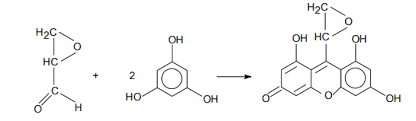
\includegraphics{reaccion kreiss.png}
\subsection{Datos experimentales} 
$Aceite$ = 2 ml \\
$HCl$ = 5,2 ml  \\
$Reactivo\ de \ Kreiss$ = 8,557 a 22,2 C  \\

\subsection{Resultados}
No se observo un cambio apreciable de coloración en la solución 




\newpage

\section{Conclusiones}
En la determinación de densidad se obtuvo un valor de 0,8681; que se encuentra fuera del rango establecido por norma; esto pudo haberse debido a la temperatura del picnometro con aceite a la hora de realizar el pesaje de la muestra. Dicho valor no se encuentra muy lejos del parámetro establecido, lo cual no es indicativo de un aceite malo.\\
Para la determinación del índice de acidez no fue necesaria la aplicación de NaOH, lo que es indicativo de que el aceite no presentaba impurezas ni degradaciones.\newline
Los resultados arrojados por la valoración hecha en el índice de yodo nos demuestra que el valor se encuentra en el rango y que el aceite tiene un nivel de pureza aceptable.\\
Por ultimo, en la prueba de rancidez por el método de Kreiss no se verifico un cambio de coloración a rojizo o rosa pálido, indicando que no se producieron cambios físico-quimicos apreciables que pudieron dañar el aceite.




\newpage
\section {Bibliografías}
\begin{itemize}
    \item {NP 14. CUERPOS GRASOS.DETERMINACIÓN DE YODO(N.D).}
    \item {NORMA PARAGUAYA NP 7 027 73. ACEITE CRUDO O VIRGEN DE GIRASOL.ESPECIFICACIONES}
    \item{NMX-F-075-SCFI-2012.ALIMENTOS – ACEITES Y GRASAS VEGETALES O ANIMALES DETERMINACIÓN DE LA DENSIDAD RELATIVA – MÉTODO DE PRUEBA}
    \item{NMX-F-101-SCFI-2012.ALIMENTOS – ACEITES Y GRASAS VEGETALES O ANIMALES – DETERMINACIÓN DE ÁCIDOS GRASOS LIBRES - MÉTODO DE PRUEBA }
    \item{NMX-F-222-1975.DETRMINACION DE RANCIDEZ EN ACEITES Y
GRASAS VEGETALES O ANIMALES.}
   
\end{itemize}



\printbibliography[
heading=bibintoc,
title={Bibliografías}
]



\end{document}
